\documentclass[aspectratio=169]{beamer}

% ── Theme ────────────────────────────────────────────────────────────────────
\usetheme{Madrid}
\usecolortheme{seahorse}
\usefonttheme{professionalfonts}
\setbeamertemplate{navigation symbols}{}
\setbeamertemplate{caption}[numbered]

% ── Packages ─────────────────────────────────────────────────────────────────
\usepackage{booktabs}
\usepackage{graphicx}
\usepackage{amsmath}
\usepackage{amssymb}
\usepackage{xcolor}
\usepackage{tikz}
\usepackage{colortbl}
\usepackage{array}
\usepackage{multirow}
\usepackage[T1]{fontenc}

% ── Custom colours ───────────────────────────────────────────────────────────
\definecolor{positive}{RGB}{33,118,174}   % steelblue
\definecolor{negative}{RGB}{192,57,43}    % tomato red
\definecolor{neutral}{RGB}{100,100,100}
\definecolor{supported}{RGB}{39,174,96}   % green
\definecolor{partial}{RGB}{243,156,18}    % orange
\definecolor{highlight}{RGB}{41,128,185}

\newcommand{\yes}{\textcolor{supported}{\checkmark}}
\newcommand{\no}{\textcolor{negative}{$\times$}}
\newcommand{\sig}[1]{\textcolor{supported}{\textbf{#1}}}
\newcommand{\ns}[1]{\textcolor{neutral}{#1}}

% ── Title info ────────────────────────────────────────────────────────────────
\title[Surprisal, Entropy \& Integration Cost]{%
  Disentangling Predictive Surprisal, Entropy,\\
  and Syntactic Integration Cost\\
  in Human Sentence Processing}
\subtitle{Mid-Project Evaluation}
\author[Gupta \& Jalan]{%
  Harshit Gupta (2022101124) \and Sanchit Jalan (2022101070)}
\date{April 2026}

% ─────────────────────────────────────────────────────────────────────────────
\begin{document}
% ─────────────────────────────────────────────────────────────────────────────

\begin{frame}
  \titlepage
\end{frame}

% ── Outline ──────────────────────────────────────────────────────────────────
\begin{frame}{Outline}
  \tableofcontents
\end{frame}

\section{Motivation}

% ── Slide 1: Core Question ───────────────────────────────────────────────────
\begin{frame}{The Core Question}

  \begin{center}
    \Large\textit{Why do some words take longer to read than others?}
  \end{center}

  \vspace{0.5em}
  \begin{columns}[T]
    \begin{column}{0.48\textwidth}
      \begin{block}{Predictive Processing}
        Unexpected words are harder to process.
        \[
          S(w_i) = -\log_2 P(w_i \mid \text{context})
        \]
        \textit{Hale 2001; Levy 2008}
      \end{block}
    \end{column}
    \begin{column}{0.48\textwidth}
      \begin{block}{Dependency Locality Theory}
        Structurally distant words are harder to integrate.
        \[
          \text{IC}(w_i) = |\text{pos}(w_i) - \text{pos}(\text{head}(w_i))|
        \]
        \textit{Gibson 2000; Demberg \& Keller 2008}
      \end{block}
    \end{column}
  \end{columns}

  \vspace{0.8em}
  \begin{alertblock}{Our Contribution}
    Test \textbf{both simultaneously} using Transformer LMs + Bayesian hierarchical
    modeling across 3 architectures and 181 readers.
  \end{alertblock}
\end{frame}

\section{Data \& Pipeline}

% ── Slide 2: Dataset ─────────────────────────────────────────────────────────
\begin{frame}{Dataset: Natural Stories Corpus}

  \begin{columns}[T]
    \begin{column}{0.55\textwidth}
      \begin{itemize}
        \item $\sim$10,000 words of English narrative text
        \item \textbf{181 participants}, self-paced reading times
        \item \textbf{835,700 total observations} after cleaning
      \end{itemize}

      \vspace{0.8em}
      \textbf{Pre-processing:}
      \begin{itemize}
        \item RT filter: 100\,ms -- 3000\,ms
        \item Per-subject $\pm3\,\sigma$ outlier removal
        \item Dependent variable: $\log(\text{RT})$
        \item Universal Dependencies parses via Stanza
      \end{itemize}
    \end{column}
    \begin{column}{0.42\textwidth}
      \begin{exampleblock}{Scale}
        \centering
        \begin{tabular}{lr}
          \toprule
          Item & Count \\
          \midrule
          Words (unique positions) & 10,245 \\
          Subjects & 181 \\
          Sentences & 485 \\
          Total observations & 835,700 \\
          After cleaning & 835,700 \\
          \bottomrule
        \end{tabular}
      \end{exampleblock}
    \end{column}
  \end{columns}
\end{frame}

% ── Slide 3: Pipeline ────────────────────────────────────────────────────────
\begin{frame}{Full Pipeline — All 6 Steps Complete}

  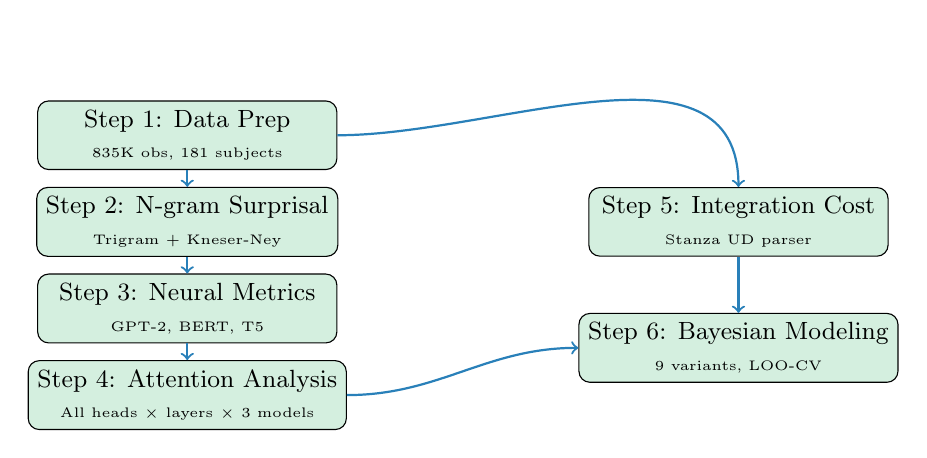
\begin{tikzpicture}[
    box/.style={draw, rounded corners, fill=highlight!15,
                minimum width=3.8cm, minimum height=0.65cm,
                font=\small, align=center},
    done/.style={box, fill=supported!20},
    arr/.style={->, thick, color=highlight}
  ]
    \node[done] (d) at (0,0)    {Step 1: Data Prep\\{\tiny 835K obs, 181 subjects}};
    \node[done] (n) at (0,-1.1) {Step 2: N-gram Surprisal\\{\tiny Trigram + Kneser-Ney}};
    \node[done] (m) at (0,-2.2) {Step 3: Neural Metrics\\{\tiny GPT-2, BERT, T5}};
    \node[done] (a) at (0,-3.3) {Step 4: Attention Analysis\\{\tiny All heads $\times$ layers $\times$ 3 models}};
    \node[done] (i) at (7,-1.1) {Step 5: Integration Cost\\{\tiny Stanza UD parser}};
    \node[done] (b) at (7,-2.7) {Step 6: Bayesian Modeling\\{\tiny 9 variants, LOO-CV}};

    \draw[arr] (d) -- (n);
    \draw[arr] (n) -- (m);
    \draw[arr] (m) -- (a);
    \draw[arr] (d.east) to[out=0,in=90] (i.north);
    \draw[arr] (i) -- (b);
    \draw[arr] (a.east) to[out=0,in=180] (b.west);
  \end{tikzpicture}

  \vspace{0.3em}
  \begin{center}
    \textcolor{supported}{\Large\checkmark}\;
    \textbf{All 6 pipeline steps complete. Results are in hand.}
  \end{center}
\end{frame}

% ── Slide 4: Bayesian model ──────────────────────────────────────────────────
\begin{frame}{Bayesian Hierarchical Model Specification}

  \[
    \log(\text{RT}_{ij}) = \alpha + u_{0i}
      + \sum_k \bigl(\beta_k + u_{ki}\bigr) X_{kj} + \varepsilon_{ij}
  \]

  \vspace{0.5em}
  \begin{columns}[T]
    \begin{column}{0.48\textwidth}
      \textbf{Priors:}
      \begin{align*}
        \alpha,\,\beta_k &\sim \mathcal{N}(0,\,1) \\
        \sigma_{u_0},\,\sigma_{\text{slope}} &\sim \text{HalfNormal}(0.5) \\
        \sigma_\varepsilon &\sim \text{HalfNormal}(0.5)
      \end{align*}
    \end{column}
    \begin{column}{0.48\textwidth}
      \textbf{9 model variants fitted:}
      \begin{itemize}\small
        \item \texttt{baseline} (trigram only)
        \item \texttt{deep\_gpt2 / bert / t5}
        \item \texttt{surprisal\_vs\_ic}
        \item \texttt{surprisal\_vs\_entropy} $\times$ 3
        \item \texttt{full} (all predictors)
      \end{itemize}
    \end{column}
  \end{columns}

  \vspace{0.5em}
  \begin{block}{Key feature}
    Random slopes for GPT-2 surprisal and IC \textbf{per subject} — enables
    quantifying individual reader strategies (H6).
  \end{block}
\end{frame}

\section{Results}

% ── Slide 5: H1 ──────────────────────────────────────────────────────────────
\begin{frame}{H1: Deep Neural Surprisal $\gg$ Shallow N-gram}

  \begin{columns}[T]
    \begin{column}{0.50\textwidth}
      \begin{table}
        \small
        \begin{tabular}{lrrl}
          \toprule
          Model & ELPD & $\beta$ & Sig.\\
          \midrule
          \rowcolor{supported!20}
          \textbf{GPT-2} & \textbf{$-$1163} & $+$0.010 & \yes \\
          T5             & $-$1191          & $+$0.013 & \yes \\
          BERT           & $-$1210          & $+$0.005 & \yes \\
          Trigram        & $-$1211          & $-$0.003 & \yes \\
          \bottomrule
        \end{tabular}
      \end{table}

      \vspace{0.5em}
      \begin{alertblock}{Finding}
        GPT-2 outperforms the trigram baseline by \textbf{48 ELPD units}.
        Human reading relies on long-distance context, not just local collocations.
      \end{alertblock}
    \end{column}
    \begin{column}{0.48\textwidth}
      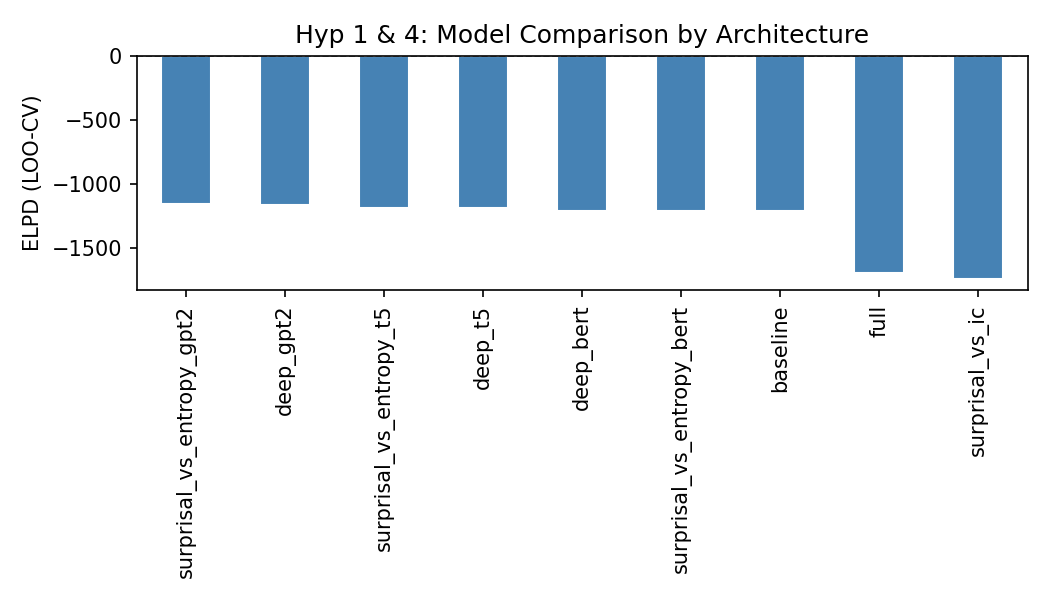
\includegraphics[width=\textwidth]{figures/figures/hyp1_deep_vs_ngram.png}
    \end{column}
  \end{columns}
\end{frame}

% ── Slide 6: H4 ──────────────────────────────────────────────────────────────
\begin{frame}{H4: Autoregressive Architecture Best Mirrors Human Reading}

  \begin{columns}[T]
    \begin{column}{0.50\textwidth}
      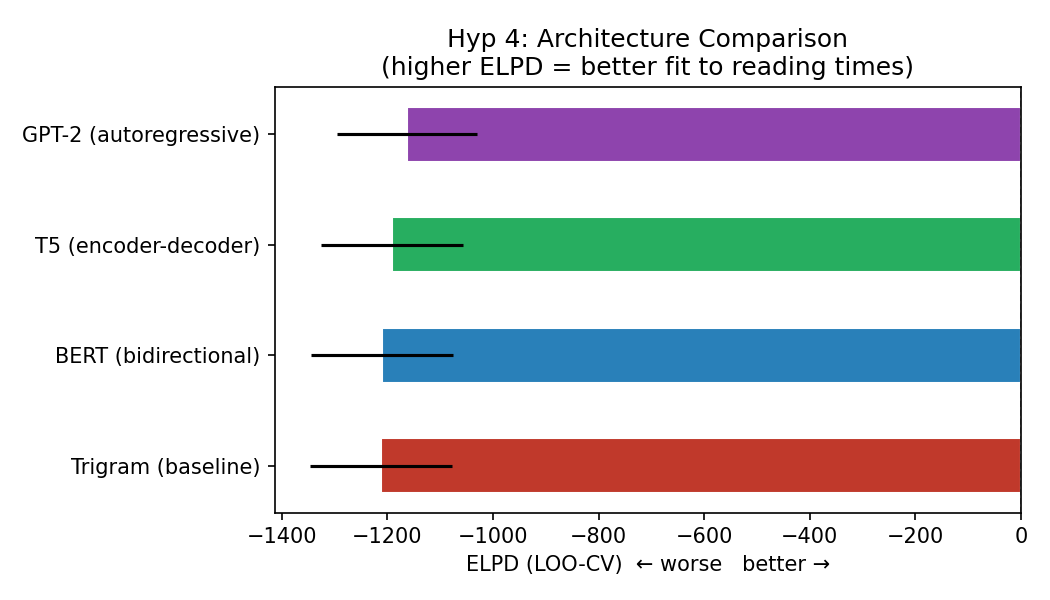
\includegraphics[width=\textwidth]{figures/figures/hyp4_architecture_comparison.png}
    \end{column}
    \begin{column}{0.48\textwidth}
      \vspace{1em}
      \begin{exampleblock}{ELPD Ranking}
        \begin{enumerate}
          \item \textbf{GPT-2} (autoregressive) $-$1163
          \item T5 (encoder-decoder) $-$1191
          \item BERT (bidirectional) $-$1210
          \item Trigram baseline $-$1211
        \end{enumerate}
      \end{exampleblock}

      \vspace{0.5em}
      \begin{alertblock}{Why BERT fails}
        Bidirectional context is unavailable during sequential human reading.
        A stronger LM is not necessarily a better psycholinguistic model.
      \end{alertblock}
    \end{column}
  \end{columns}
\end{frame}

% ── Slide 7: H2 ──────────────────────────────────────────────────────────────
\begin{frame}{H2: Integration Cost Explained Away by Neural Surprisal}

  \begin{columns}[T]
    \begin{column}{0.50\textwidth}
      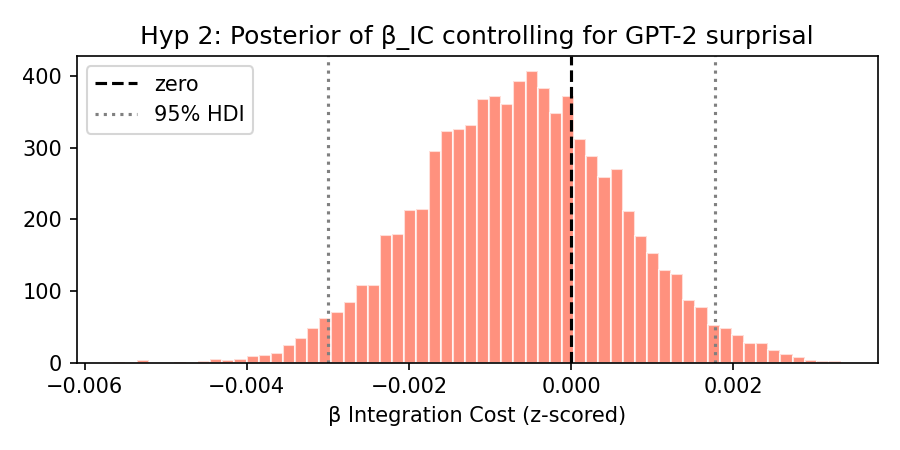
\includegraphics[width=\textwidth]{figures/figures/hyp2_ic_variance_explained.png}
    \end{column}
    \begin{column}{0.48\textwidth}
      \vspace{0.5em}
      \begin{table}
        \small
        \begin{tabular}{lrll}
          \toprule
          Predictor & $\beta$ & 95\% HDI & Sig.\\
          \midrule
          GPT-2 surprisal  & $+$0.014 & [$+$0.011,\,$+$0.018] & \yes \\
          Integration cost & $-$0.001 & [$-$0.003,\,$+$0.002] & \no  \\
          \bottomrule
        \end{tabular}
      \end{table}

      \vspace{0.5em}
      \begin{alertblock}{Finding}
        The posterior for $\beta_{\text{IC}}$ spans zero symmetrically.
        Neural surprisal \textbf{fully subsumes} the variance previously
        attributed to structural memory load.
      \end{alertblock}
    \end{column}
  \end{columns}
\end{frame}

% ── Slide 8: H3 ──────────────────────────────────────────────────────────────
\begin{frame}{H3: Surprisal and Entropy are Partly Independent}

  \begin{columns}[T]
    \begin{column}{0.52\textwidth}
      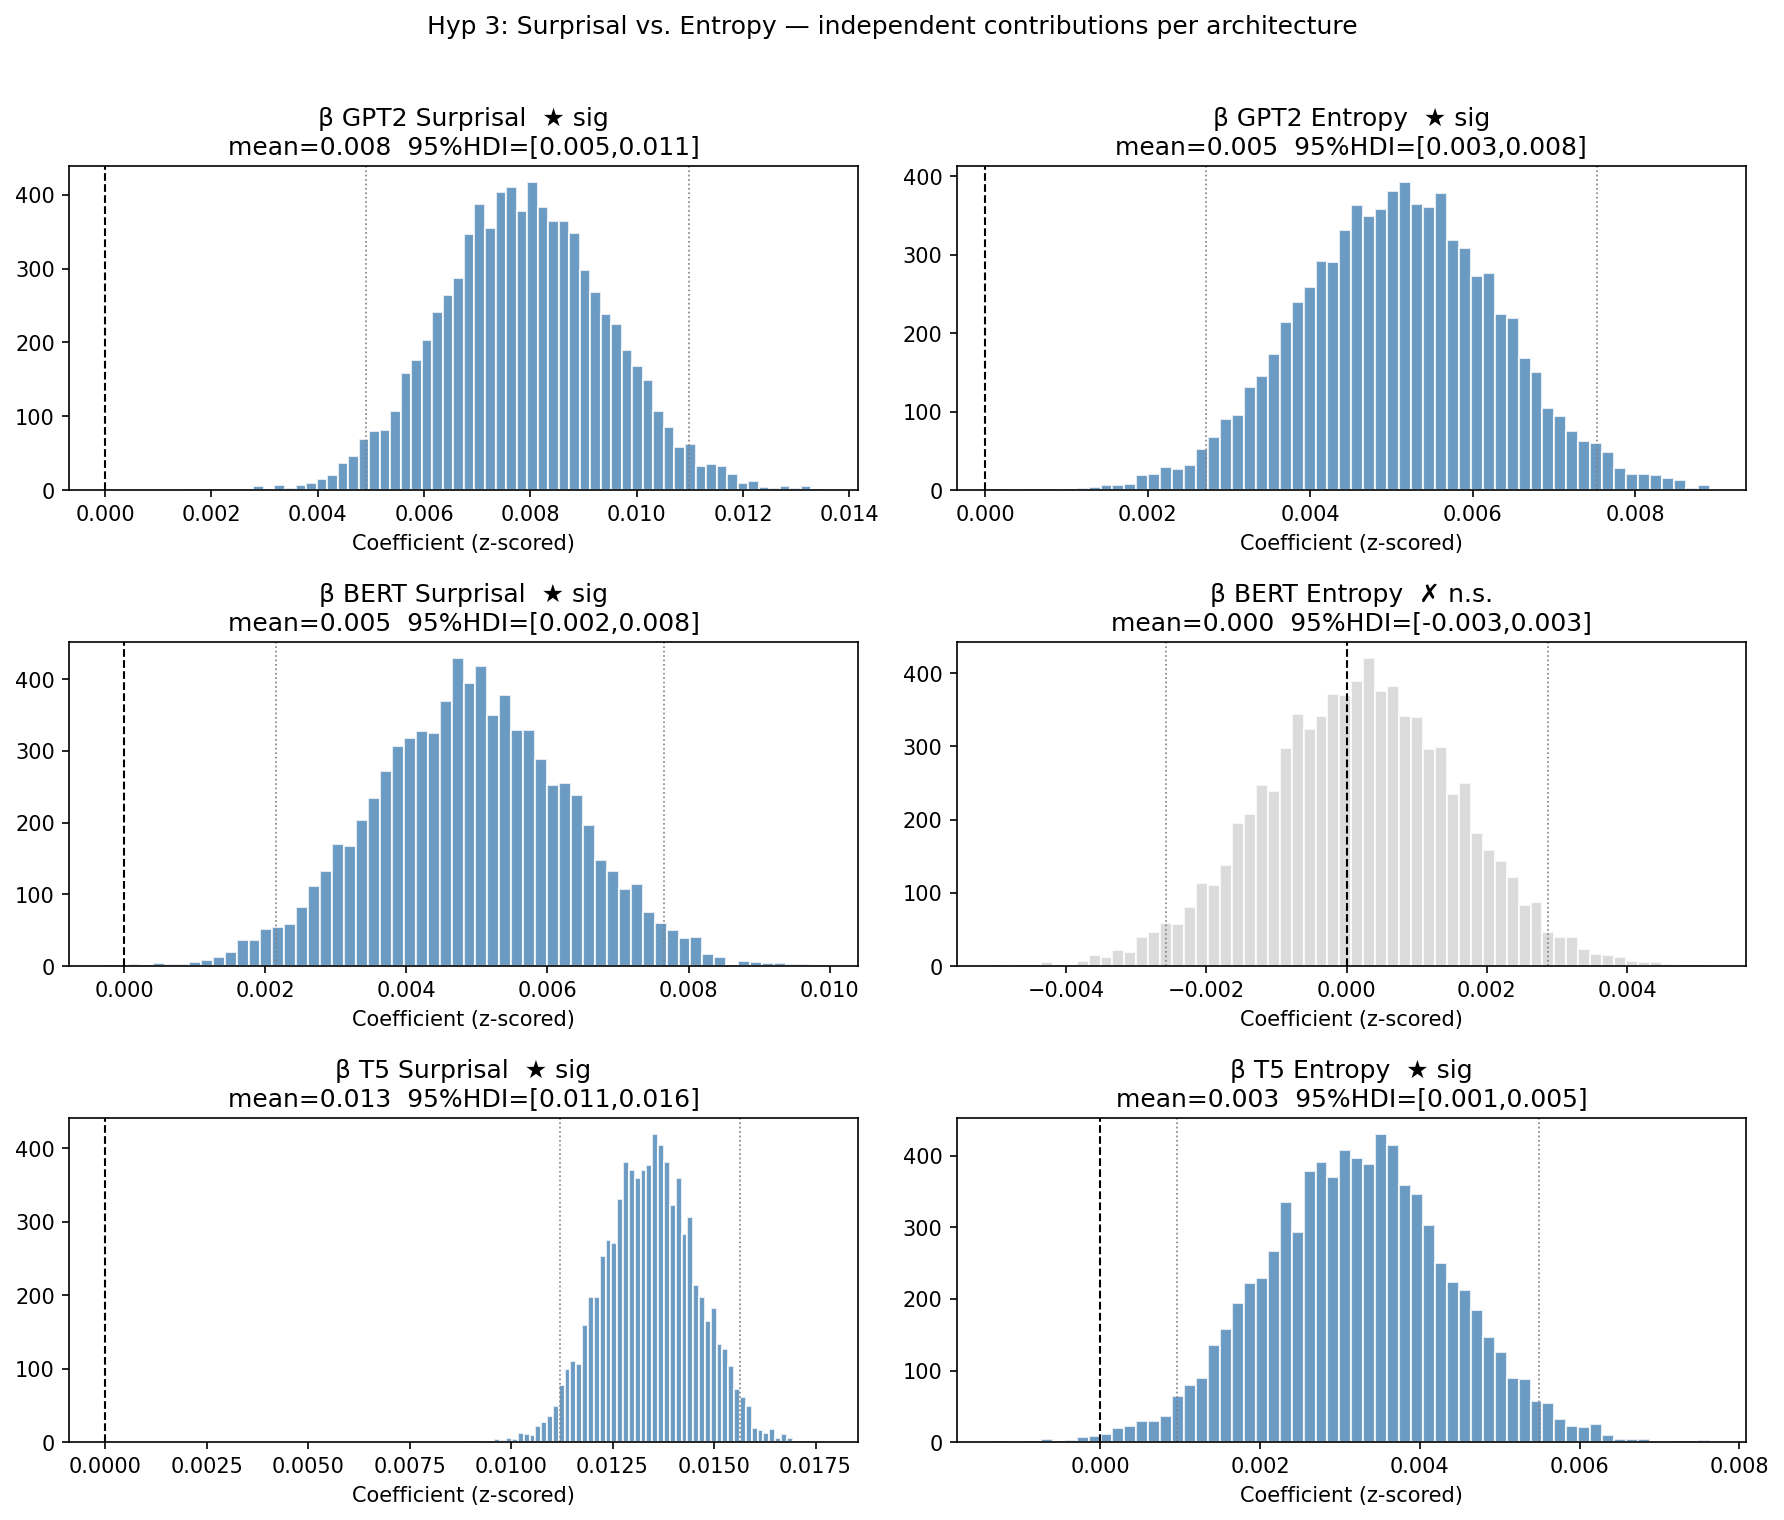
\includegraphics[width=\textwidth]{figures/figures/hyp3_surprisal_vs_entropy.png}
    \end{column}
    \begin{column}{0.46\textwidth}
      \vspace{0.5em}
      \begin{table}
        \small
        \begin{tabular}{lll}
          \toprule
          Arch. & $\beta_{\text{surp}}$ & $\beta_{\text{entr}}$ \\
          \midrule
          GPT-2 & $+$0.008 \yes & $+$0.005 \yes \\
          T5    & $+$0.013 \yes & $+$0.003 \yes \\
          BERT  & $+$0.005 \yes & $+$0.000 \no  \\
          \bottomrule
        \end{tabular}
      \end{table}

      \vspace{0.4em}
      \begin{block}{Interpretation}
        GPT-2 \& T5: knowing the model was \textit{uncertain} predicts
        reading difficulty \emph{beyond} just the specific word's probability.\\[0.3em]
        BERT entropy is non-informative — bidirectional pseudo-surprisal
        conflates the two measures.
      \end{block}
    \end{column}
  \end{columns}
\end{frame}

% ── Slide 9: H5 overview ─────────────────────────────────────────────────────
\begin{frame}{H5: Specific Attention Heads Track Syntactic Structure}

  \begin{columns}[T]
    \begin{column}{0.50\textwidth}
      \begin{table}
        \small
        \begin{tabular}{llrl}
          \toprule
          Architecture & Best Head & $\rho$ & $p$-value \\
          \midrule
          BERT  & L0\,H10 & \sig{$-$0.624} & $<10^{-100}$ \\
          T5    & L0\,H10 & \sig{$-$0.579} & $<10^{-100}$ \\
          GPT-2 & L5\,H9  & $+$0.351       & $<10^{-100}$ \\
          \bottomrule
        \end{tabular}
      \end{table}

      \vspace{0.4em}
      \begin{alertblock}{Convergent finding}
        \textbf{The same head (L0\,H10) dominates in both BERT and T5},
        despite different training objectives — a convergent structural inductive bias.
      \end{alertblock}
    \end{column}
    \begin{column}{0.48\textwidth}
      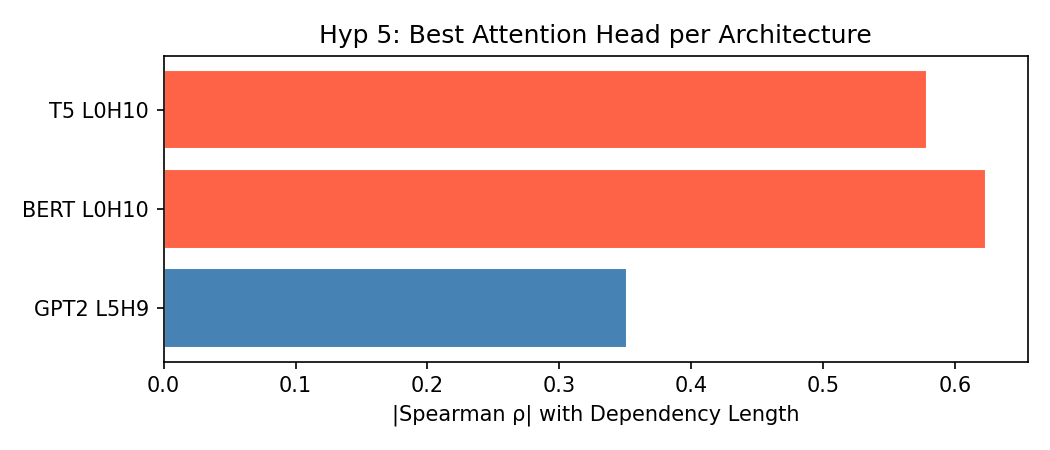
\includegraphics[width=\textwidth]{figures/figures/hyp5_attention_comparison.png}
    \end{column}
  \end{columns}
\end{frame}

% ── Slide 10: H5 deep dive ───────────────────────────────────────────────────
\begin{frame}{H5 Deep Dive: BERT L0\,H10 Head-Finding Accuracy}

  \begin{columns}[T]
    \begin{column}{0.50\textwidth}
      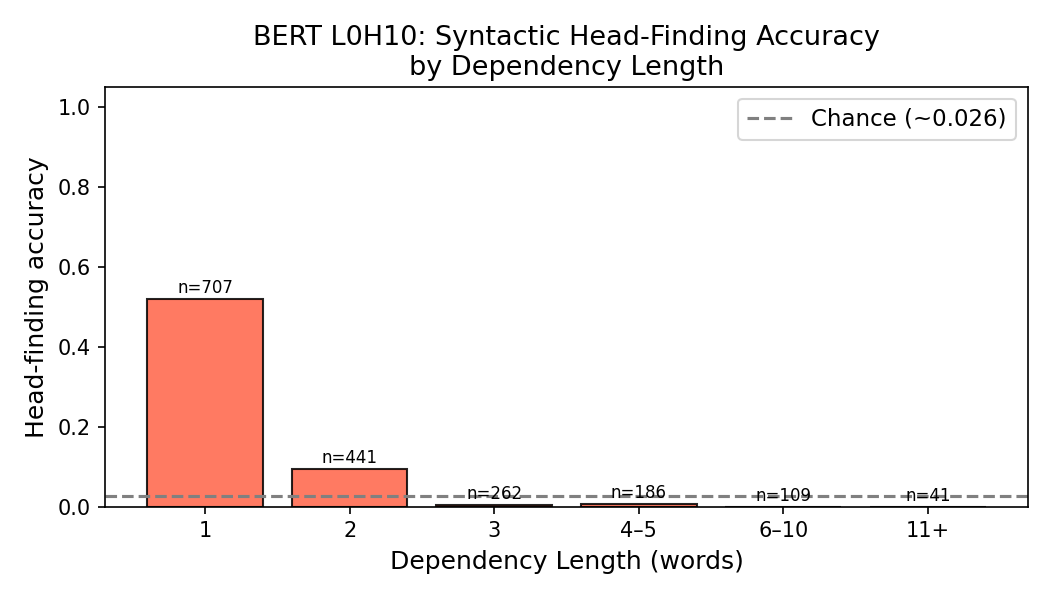
\includegraphics[width=\textwidth]{figures/figures/bert_L0H10_headfinding_accuracy.png}
    \end{column}
    \begin{column}{0.48\textwidth}
      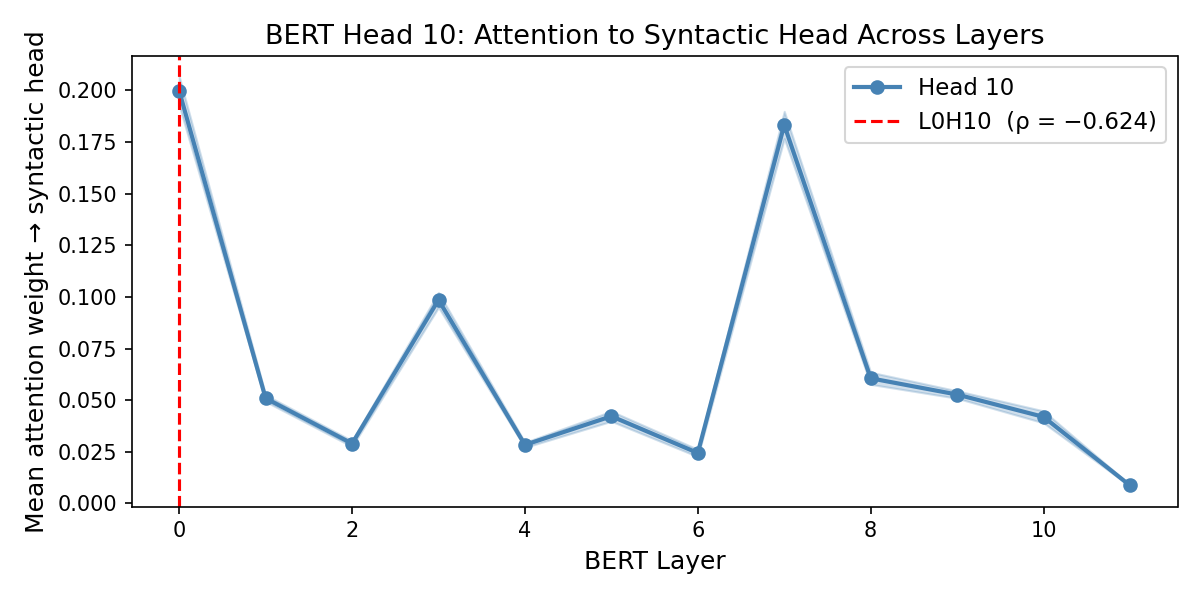
\includegraphics[width=\textwidth]{figures/figures/bert_L0H10_layer_curve.png}
    \end{column}
  \end{columns}

  \vspace{0.3em}
  \begin{block}{Interpretation}
    Head-finding accuracy: $\approx$60\% for DL$=$1, drops to $\approx$15\%
    for DL$>$5 (near chance). Layer 0 has the \emph{highest} mean attention
    to syntactic heads, declining in deeper layers — a local structural bias
    that mirrors the human working memory constraint.
  \end{block}
\end{frame}

% ── Slide 11: H6 ─────────────────────────────────────────────────────────────
\begin{frame}{H6: Individual Reader Strategies}

  \begin{columns}[T]
    \begin{column}{0.52\textwidth}
      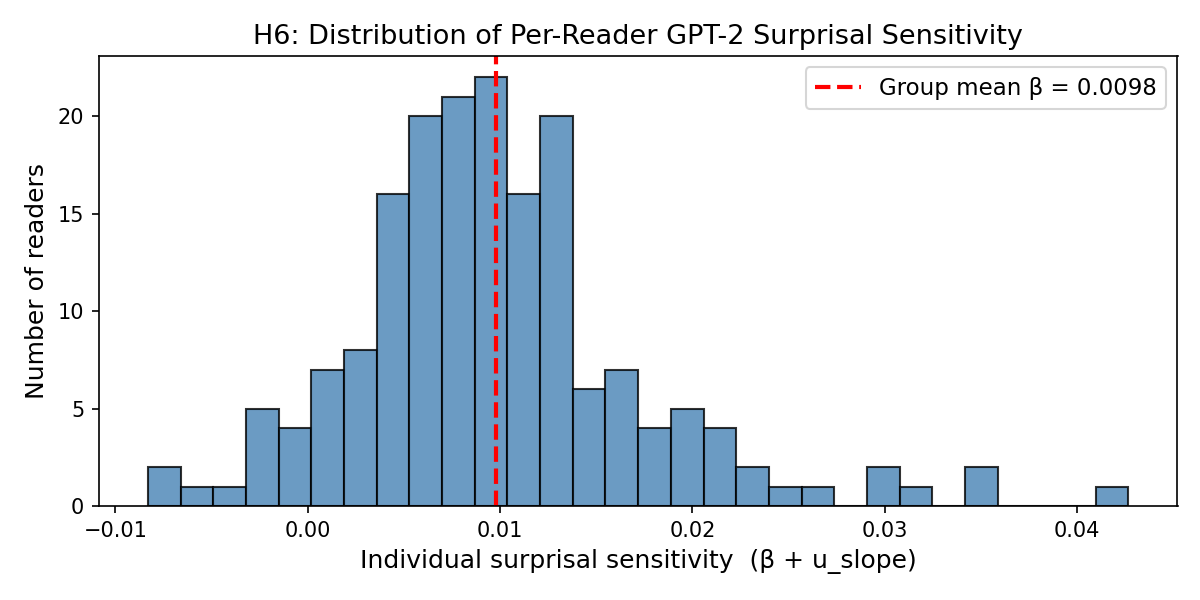
\includegraphics[width=\textwidth]{figures/figures/H6_surprisal_slopes_hist.png}
    \end{column}
    \begin{column}{0.46\textwidth}
      \vspace{0.5em}
      \begin{table}
        \small
        \begin{tabular}{lrll}
          \toprule
          Component & $\sigma$ & 95\% HDI & Sig.\\
          \midrule
          Surprisal slope & \textbf{0.013} & [0.009,\,0.016] & \yes \\
          IC slope        & 0.003          & [0.000,\,0.007] & \yes \\
          \bottomrule
        \end{tabular}
      \end{table}

      \vspace{0.4em}
      \begin{alertblock}{Finding}
        $\sigma_{\text{slope}} > 0$: genuine between-reader variation in
        surprisal sensitivity. Some readers slow sharply at unexpected words;
        others are barely affected. This heterogeneity is invisible to
        standard LMER models.
      \end{alertblock}
    \end{column}
  \end{columns}
\end{frame}

\section{Summary}

% ── Slide 12: Hypothesis summary ─────────────────────────────────────────────
\begin{frame}{Summary: All 6 Hypotheses Tested}

  \begin{table}
    \renewcommand{\arraystretch}{1.3}
    \begin{tabular}{llp{6cm}}
      \toprule
      \textbf{Hyp.} & \textbf{Status} & \textbf{Key Finding} \\
      \midrule
      H1: Deep $>$ Shallow
        & \textcolor{supported}{\textbf{Supported}}
        & GPT-2 $\Delta$ELPD $= +48$ over trigram \\
      H2: Surprisal subsumes IC
        & \textcolor{supported}{\textbf{Supported}}
        & $\beta_{\text{IC}}$ HDI spans zero \\
      H3: Surprisal $\neq$ Entropy
        & \textcolor{partial}{\textbf{Partial}}
        & GPT-2 \& T5 yes; BERT entropy n.s. \\
      H4: Autoregressive best
        & \textcolor{supported}{\textbf{Supported}}
        & GPT-2 $>$ T5 $>$ BERT $\approx$ trigram \\
      H5: Heads track syntax
        & \textcolor{supported}{\textbf{Strongly}}
        & $\rho = -0.624$ (BERT L0\,H10) \\
      H6: Individual differences
        & \textcolor{supported}{\textbf{Supported}}
        & $\sigma_{\text{slope}} = 0.013$, credibly $> 0$ \\
      \bottomrule
    \end{tabular}
  \end{table}

  \vspace{0.3em}
  \begin{center}
    \textbf{5 of 6 fully supported \; · \; 1 partially supported}
  \end{center}
\end{frame}

% ── Slide 13: Work remaining ─────────────────────────────────────────────────
\begin{frame}{Work Remaining}

  \begin{columns}[T]
    \begin{column}{0.48\textwidth}
      \begin{exampleblock}{Completed \checkmark}
        \begin{itemize}
          \item Full 6-step pipeline
          \item GPT-2, BERT, T5 surprisal \& entropy
          \item T5 attention head analysis (new)
          \item 9 Bayesian model variants
          \item LOO-CV model comparison
          \item All 6 hypotheses tested \& visualised
          \item Individual reader slope analysis
        \end{itemize}
      \end{exampleblock}
    \end{column}
    \begin{column}{0.48\textwidth}
      \begin{alertblock}{Remaining for Final}
        \begin{enumerate}
          \item \textbf{GECO corpus} — cross-dataset validation on eye-tracking data (54K words)
          \item \textbf{Final report} — full statistical write-up
          \item \textbf{MCMC robustness} — address intercept mixing for hierarchical models
        \end{enumerate}
      \end{alertblock}
    \end{column}
  \end{columns}
\end{frame}

% ── Slide 14: Takeaways ──────────────────────────────────────────────────────
\begin{frame}{Key Takeaways}

  \begin{enumerate}
    \setlength\itemsep{0.6em}
    \item \textbf{Neural LMs $\gg$ N-grams} for predicting reading difficulty —
          long-distance context is essential.

    \item \textbf{Architecture modality matters} — left-to-right GPT-2 best
          mirrors the incremental human reading process.

    \item \textbf{Structural memory load is not independently necessary} —
          neural surprisal already encodes dependency-based difficulty.

    \item \textbf{Transformers implicitly learn syntax} — the same head
          (L0\,H10) tracks dependency structure in both BERT and T5,
          suggesting a convergent structural inductive bias.

    \item \textbf{Reading is not one-size-fits-all} — Bayesian modeling
          reveals meaningful individual differences in predictive processing
          that standard LMERs miss.
  \end{enumerate}
\end{frame}

% ── References ───────────────────────────────────────────────────────────────
\begin{frame}{References}
  \footnotesize
  \begin{enumerate}
    \item Hale, J. (2001). A probabilistic Earley parser as a psycholinguistic model. \textit{NAACL}.
    \item Levy, R. (2008). Expectation-based syntactic comprehension. \textit{Cognition}, 106(3).
    \item Demberg, V. \& Keller, F. (2008). Data from eye-tracking corpora as evidence for theories of syntactic processing complexity. \textit{Cognition}, 109(2).
    \item Oh, B. \& Schuler, W. (2023). Transformer-based Language Models Explain Human Reading Times. \textit{CogSci}.
    \item Wilcox, E. G. et al. (2020). On the Predictive Power of Neural Language Models for Human Real-Time Comprehension Behavior. \textit{CogSci}.
    \item Clark, K. et al. (2019). What Does BERT Look At? An Analysis of BERT's Attention. \textit{BlackboxNLP}.
  \end{enumerate}
\end{frame}

\end{document}
